\documentclass[11pt,a4paper]{article}
\usepackage[T1]{fontenc}
\usepackage[utf8]{inputenc}
\usepackage{lmodern}
\usepackage[margin=2.5cm]{geometry}
\usepackage{amsmath,amssymb}
\usepackage{booktabs}
\usepackage{graphicx}
\usepackage[hidelinks]{hyperref}
\hypersetup{pdfauthor={Gianni Pilotti},pdftitle={Rebuilding the ECB Euro Area Yield Curve},pdfcreator={},pdfproducer={}}
\setlength{\parindent}{0pt}
\setlength{\parskip}{6pt}

\title{Rebuilding the ECB Euro Area Yield Curve}
\author{Gianni Pilotti}
\date{}

\begin{document}
\maketitle

\section{The Core Idea}

The ECB publishes two things each day: the six parameters of a Svensson curve, and the spot, forward and par yield curves computed from them. If the formulas are right, rebuilding the rates from the parameters gives the published numbers exactly. That is a clean test of a curve implementation, and it is the starting point of the project.

Once the curve is reproduced, it is used for three tasks:

\begin{itemize}
\item \textbf{Bond risk:} price a bullet bond off the curve and measure duration, DV01 and key rate durations.
\item \textbf{Factor structure:} a principal component analysis (PCA) of daily curve moves.
\item \textbf{Relative value:} butterflies on the curve that carry no level or slope exposure, tested in a backtest after costs.
\end{itemize}

The data are the ECB curves from 2004 to 2026.

\section{Method}

\subsection{Svensson Curve}

With $\beta_0,\dots,\beta_3,\tau_1,\tau_2$ the ECB parameters, the code (\texttt{eyc/svensson.py}) uses continuously compounded rates in percent. With $x_i=t/\tau_i$:
\begin{equation}
f(t)=\beta_0+\beta_1e^{-x_1}+\beta_2x_1e^{-x_1}+\beta_3x_2e^{-x_2},
\end{equation}
\begin{equation}
y(t)=\beta_0+\beta_1\frac{1-e^{-x_1}}{x_1}+\beta_2\Big(\frac{1-e^{-x_1}}{x_1}-e^{-x_1}\Big)+\beta_3\Big(\frac{1-e^{-x_2}}{x_2}-e^{-x_2}\Big),
\end{equation}
\begin{equation}
DF(t)=e^{-y(t)\,t}.
\end{equation}
The spot rate $y$ is the average of the forward rate $f$ over $[0,t]$.

\subsection{Par Yield}

The ECB defines the par yield against a continuous annuity:
\begin{equation}
y_{\text{par}}(T)=100\cdot\frac{1-DF(T)}{\int_0^T DF(t)\,dt}.
\end{equation}
The integral is evaluated with 64-point Gauss--Legendre quadrature. Before 19 May 2023 the ECB used a monthly sum of discount factors instead of the integral and did not restate the history, so the code implements both and picks one by date.

\subsection{Bond Risk}

A bond's dirty price is the sum of its cash flows discounted with $DF$. Curve risk uses a $\pm1$ bp parallel shift, applied exactly by bumping $\beta_0$:
\begin{equation}
\text{DV01}=\frac{P_{-}-P_{+}}{2},\qquad
D_{\text{eff}}=\frac{P_{-}-P_{+}}{2P\cdot 10^{-4}}.
\end{equation}
Key rate durations bump the zero curve with triangular weights on the tenors 0.5, 2, 5, 10 and 30 years. The weights sum to one at every maturity, so the key rate durations add up to $D_{\text{eff}}$. A test checks this identity.

\subsection{PCA and Neutral Butterflies}

The PCA uses daily spot changes. Loadings are fitted on the first half of the sample and scored on the second half. For a butterfly on three maturities with loadings $L$ on level and slope, the weights $w$ solve
\begin{equation}
L_{\text{level}}^{\top}w=0,\qquad L_{\text{slope}}^{\top}w=0,
\end{equation}
with the belly weight fixed at one. The solution is the null space of a $2\times3$ matrix, found with an SVD. Loadings come from a trailing 250-day window and the weights are reset every 21 days.

The signal is a z-score of the structure against its trailing 120-day mean and standard deviation, scored at today's weights so that a weight reset does not create a false signal. A position opens at $|z|>1.5$ and closes at $|z|<0.5$. The position taken on day $t$ earns the move from $t$ to $t+1$. Cost is 0.5 bp round trip per unit of DV01 traded.

\section{Results}

\subsection{Curve Reconstruction}

Maximum error against the published rates, in basis points (all-issuers: 5,614 dates, 120 maturities).

\begin{center}
\begin{tabular}{llrr}
\toprule
Curve & Rate & Max error & Dates above 0.01 bp \\
\midrule
All issuers & Spot & $1.5\times10^{-8}$ & 0 \\
All issuers & Par yield & $2.8\times10^{-7}$ & 0 \\
AAA & Spot & 5.6 & 1 \\
AAA & Par yield & 7.4 & 2 \\
\bottomrule
\end{tabular}
\end{center}

\begin{itemize}
\item \textbf{Compounding:} treating the rates as annually compounded gives a 6.9 bp error at 10 years.
\item \textbf{Par yield:} dividing by an annual coupon schedule instead of the continuous annuity is off by 6.8 bp at 10 years.
\item \textbf{Methodology change:} 4,782 dates match the monthly formula and 832 match the integral. None match both.
\item \textbf{AAA errors:} they come from three dates where the ECB's own AAA parameters and published rates disagree.
\end{itemize}

\subsection{Curve Analysis}

Three PCA factors explain 96.0\% of the variance of daily changes in sample and 98.6\% out of sample. The mean 10-year spread between the all-issuers and AAA curves is 55.4 bp, with a peak of 194.8 bp on 23 July 2012. For a 30-year bond with a 2\% coupon on the latest curve, the effective duration is 20.11 years, and 16.17 years of it sit in the 30-year bucket. A 10-year hedge covers only 3.14 years of it.

\subsection{Butterfly Backtest}

Five butterflies, 2005--2026, net of costs.

\begin{center}
\begin{tabular}{lrrr}
\toprule
Structure & Net P\&L (bp) & Sharpe & t-stat \\
\midrule
2s5s10s   & 108 & 0.13 & 0.59 \\
5s10s30s  & 335 & 0.30 & 1.40 \\
3s7s15s   & 279 & 0.31 & 1.43 \\
2s10s30s  & 168 & 0.14 & 0.62 \\
1s3s7s    & $-305$ & $-0.35$ & $-1.61$ \\
Portfolio & 117 & 0.16 & 0.75 \\
\bottomrule
\end{tabular}
\end{center}

No t-statistic exceeds 2. The result is not statistically significant. Costs matter more than the signal: trading the z-score continuously instead of with entry and exit bands raises turnover from about 11 to about 70 times a year.

\begin{figure}[ht]
\centering
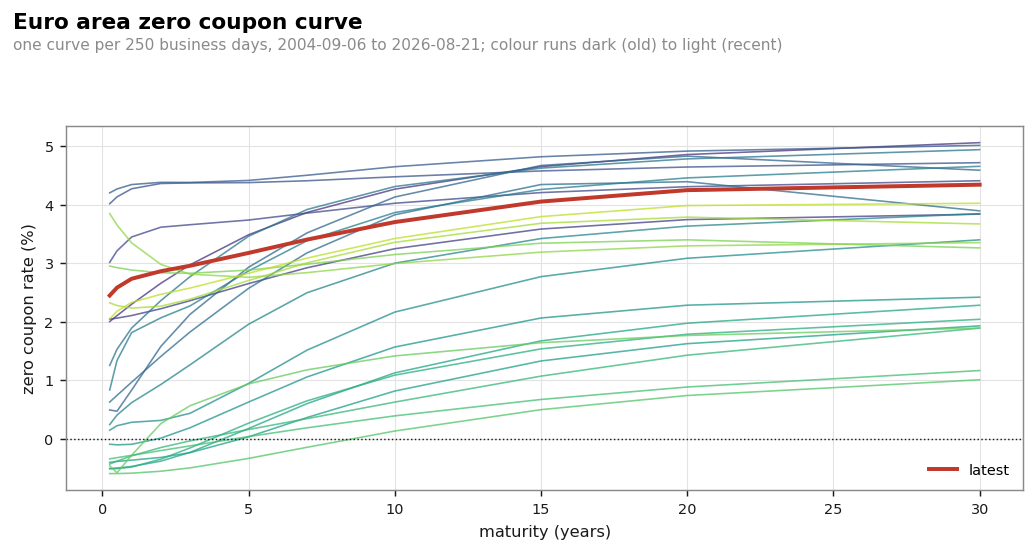
\includegraphics[width=0.85\textwidth]{../output/figures/01_curve_history.png}
\caption{Euro area zero coupon curve, one curve per 250 business days.}
\end{figure}

\section{Worked Example}

The Svensson parameters are illustrative: $\beta=(3.0,-1.5,2.0,-1.0)$, $\tau_1=2$, $\tau_2=6$.

\textbf{Spot and discount factor at 10 years.} The code gives $y(10)=2.7881\%$, so $DF(10)=e^{-0.027881\cdot10}=0.75669$.

\textbf{Annuity.} The Gauss--Legendre integral of $DF(t)$ over $[0,10]$ is 8.7462.

\textbf{Par yield.} $y_{\text{par}}(10)=100\cdot(1-0.75669)/8.7462=2.7819\%$. The monthly-sum version gives 2.7852\%, a gap of 0.33 bp between the two conventions on this curve.

\textbf{10-year bond.} A 2\% annual coupon bond has a dirty price of 92.917. Its effective duration is 9.1206, so $\text{DV01}=92.917\cdot9.1206\cdot10^{-4}=0.0847$ per 100 face.

\textbf{Butterfly weights.} Take illustrative loadings for the 2, 5 and 10-year points: level $(0.40,0.35,0.30)$ and slope $(-0.60,-0.10,0.45)$. With weights $(a,1,b)$:
\begin{align*}
0.40a+0.35+0.30b&=0,\\
-0.60a-0.10+0.45b&=0.
\end{align*}
The first gives $a=-0.875-0.75b$. Substituting, $0.425+0.9b=0$, so $b=-0.4722$ and $a=-0.5208$. The code returns the same weights $(-0.5208,\,1,\,-0.4722)$. The structure is flat to level and slope. Its gross DV01 is $0.5208+1+0.4722=1.993$ per unit of belly.

\section{Limits}

\begin{itemize}
\item \textbf{Government curve:} it is not a swap or OIS curve, so it cannot discount collateralised derivatives.
\item \textbf{Parameters not re-estimated:} the euro parameters are the ECB's, because the bond prices behind them are not public. The fitting step is tested on US data only.
\item \textbf{No calendar:} cash flows are placed at exact year fractions.
\item \textbf{Curve points, not instruments:} the backtest trades points on a fitted curve, with a flat 0.5 bp cost. Real futures or swaps would add basis and financing.
\item \textbf{No edge shown:} the portfolio t-statistic is 0.75. The backtest is a method check, not evidence of a tradable strategy.
\end{itemize}

\end{document}
